\setAuthor{Jaak Kikas}
\setRound{lõppvoor}
\setYear{2008}
\setNumber{G 5}
\setDifficulty{4}
\setTopic{Geomeetriline optika}

\prob{Veealune valgus}
Kas basseini kohal rippuv punktvalgusallikas, mida vaadeldakse basseini põhjast, on heledam siis, kui bassein on veest tühi, või siis, kui ta on veega täidetud ja kaugus silmast veepinnani võrdub valgusallika kõrgusega veepinna kohal? Mitu korda? Veepinnalt peegeldub tagasi $r = \SI{2}{\%}$ valgust, vee murdumisnäitaja on $n = \num{1,33}$ ja neeldumine vees on tühine. Allika heledus on võrdeline silmaavasse sattuva valguse energiaga, silmaava läbimõõdu loeme samaks kõigis vaatlustingimustes ja väikeseks võrreldes vaatleja sügavusega.

\hint
Allika heledus on ligikaudselt võrdeline vaatleja silmaava nurkläbimõõdu ruuduga allika asukohast vaadatuna.

\solu
\begin{wrapfigure}{r}{0.5\textwidth}
	\begin{center}
		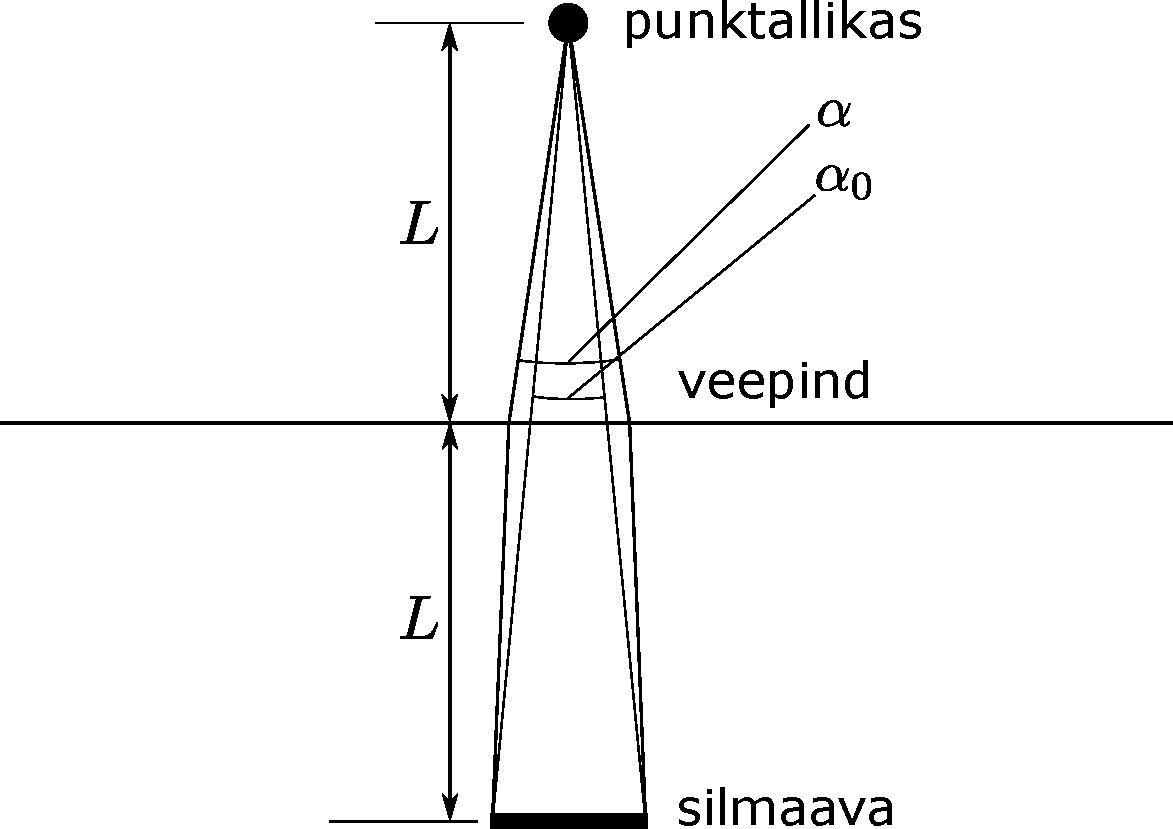
\includegraphics[width=0.95\linewidth]{2008-v3g-05-lah}
	\end{center}
\end{wrapfigure}
Allika heledus on ligikaudselt võrdeline vaatleja silmaava nurkläbimõõdu ruuduga allika asukohast vaadatuna. Olgu $\alpha$ ja $\alpha_0$ nurkläbimõõdud vastavalt veega täidetud ja veeta basseinis.

Jooniselt
\[
2L\tan (\alpha_0 /2) = L\tan (\alpha /2) + L\tan (\beta /2),
\]
kus langemis- ja murdumisnurkade $\alpha /2$ ja $\beta /2$ vahel kehtib seos
\[
\frac{\sin(\alpha/2)}{\sin(\beta/2)} = n.
\]
Kasutades väikeste nurkade lähendust $\tan\alpha\approx\sin\alpha\approx\alpha$, saame 
\[
\left(\frac{\alpha}{\alpha_0}\right)^2 = \frac{4n^2}{(n+1)^2}.
\]
Arvestades ka peegeldumist veepinnalt, saame heleduste suhteks
\[
\frac{I}{I_{0}}=\left(\frac{\alpha}{\alpha_0}\right)^2(1-r) = \frac{4(1-r) n^{2}}{(n+1)^{2}}=\num{1,28}.
\]
\probend